\documentclass[a4paper,11pt]{article}
\usepackage{amsmath,amsthm,amsfonts,amssymb,amscd,amstext,vmargin,graphics,graphicx,tabularx,multicol} 
\usepackage[francais]{babel}
\usepackage[utf8]{inputenc}  
\usepackage[T1]{fontenc} 
\usepackage{pstricks-add,tikz,tkz-tab,variations}
\usepackage[autolanguage,np]{numprint} 
\usepackage{calc}
\usepackage{pifont}

\setmarginsrb{1.5cm}{0.5cm}{1cm}{0.5cm}{0cm}{0cm}{0cm}{0cm} %Gauche, haut, droite, haut
\newcounter{numexo}
\newcommand{\exo}[1]{\stepcounter{numexo}\noindent{\bf Exercice~\thenumexo} : }
\reversemarginpar

\newcommand{\bmul}[1]{\begin{multicols}{#1}}
\newcommand{\emul}{\end{multicols}}

\newcounter{enumtabi}
\newcounter{enumtaba}
\newcommand{\q}{\stepcounter{enumtabi} \theenumtabi.  }
\newcommand{\qa}{\stepcounter{enumtaba} (\alph{enumtaba}) }
\newcommand{\initq}{\setcounter{enumtabi}{0}}
\newcommand{\initqa}{\setcounter{enumtaba}{0}}

\newcommand{\be}{\begin{enumerate}}
\newcommand{\ee}{\end{enumerate}}
\newcommand{\bi}{\begin{itemize}}
\newcommand{\ei}{\end{itemize}}
\newcommand{\bp}{\begin{pspicture*}}
\newcommand{\ep}{\end{pspicture*}}
\newcommand{\bt}{\begin{tabular}}
\newcommand{\et}{\end{tabular}}
\renewcommand{\tabularxcolumn}[1]{>{\centering}m{#1}} %(colonne m{} centrée, au lieu de p par défault) 
\newcommand{\tnl}{\tabularnewline}

\newcommand{\trait}{\noindent \rule{\linewidth}{0.2mm}}
\newcommand{\hs}[1]{\hspace{#1}}
\newcommand{\vs}[1]{\vspace{#1}}

\newcommand{\N}{\mathbb{N}}
\newcommand{\Z}{\mathbb{Z}}
\newcommand{\R}{\mathbb{R}}
\newcommand{\C}{\mathbb{C}}
\newcommand{\Dcal}{\mathcal{D}}
\newcommand{\Ccal}{\mathcal{C}}
\newcommand{\mc}{\mathcal}

\newcommand{\vect}[1]{\overrightarrow{#1}}
\newcommand{\ds}{\displaystyle}
\newcommand{\eq}{\quad \Leftrightarrow \quad}
\newcommand{\vecti}{\vec{\imath}}
\newcommand{\vectj}{\vec{\jmath}}
\newcommand{\Oij}{(O;\vec{\imath}, \vec{\jmath})}
\newcommand{\OIJ}{(O;I,J)}


\newcommand{\reponse}[1][1]{%
\multido{}{#1}{\makebox[\linewidth]{\rule[0pt]{0pt}{20pt}\dotfill}
}}

\newcommand{\titre}[5] 
% #1: titre #2: haut gauche #3: bas gauche #4: haut droite #5: bas droite
{
\noindent #2 \hfill #4 \\
#3 \hfill #5

\vspace{-1.6cm}

\begin{center}\rule{6cm}{0.5mm}\end{center}
\vspace{0.2cm}
\begin{center}{\large{\textbf{#1}}}\end{center}
\begin{center}\rule{6cm}{0.5mm}\end{center}
}



\begin{document}
\pagestyle{empty}
\titre{Séance d'AP . . . : Factorisation}{}{}{3ème}{}

\vspace*{0.2cm}


\setlength{\fboxrule}{2pt}
\begin{flushleft}
\framebox{\begin{minipage}{\linewidth}

\vspace*{0.2cm}

\underline{\textbf{{\large Rappels :}}}\\


\ding{228} Pour \textbf{factoriser}, il faut trouver dans l'expression \textbf{un facteur commun}.\\

\textbf{\underline{Exemples : }}

\bmul{3}

$7x-10x^{2}= $


\columnbreak

$5x^{3}+ 25x -10 =$


\columnbreak

$42x^{3} + 6x= $

\emul




\vspace*{1.25cm}

\textbf{Un peu plus dur !}
\bmul{2}

$E= \textbf{(9x-4)}(5x+6)+\textbf{(9x-4)}(3x+11)$\\
$E= \textbf{(9x-4)}[(5x+6)+(3x+11)]$\\
$E= \textbf{(9x-4)}[5x+6+3x+11]$\\
$E= \textbf{(9x-4)}[8x+17]$\\

\columnbreak

$B=\textbf{(3x-2)}(5-7x)-(8x+3)\textbf{(3x-2)}$\\
$B=\textbf{(3x-2)}[(5-7x)-(8x+3)]$\\
$B=\textbf{(3x-2)}[5-7x-8x-3)]$\\
$B=\textbf{(3x-2)}[2-15x)]$\\

\emul

\end{minipage}}
\end{flushleft}


\vspace*{0.5cm}

\exo \\
Surligner les expressions qui sont factorisées :\\

\includegraphics[scale=0.7]{factorisationap1.eps} \\


\exo \\
Factoriser chaque expression suivante :

\bmul{3}

$A=4a^{2}-3a$\\
\reponse[2]\\

$L=3t + 9u + 3$\\
\reponse[2]\\

\columnbreak

$G=18b-6b^{2}$ \\
\reponse[2]\\

$M= 14x+4x^{2}-22x^{3}$\\
\reponse[2]\\

\columnbreak

$D=31x-31$\\
\reponse[2]\\

$P=3x^{4}+2x^{2}$\\
\reponse[2]\\

\emul

\exo \\
 Factorisations (niveau 3ème) : Surligner le facteur commun puis factoriser.

\bmul{2}

$I=(x+2)(2x-1)+(x+2)(3x-5)$
\reponse[4]

\columnbreak

$S=(5x-3)(x-7)+(x-7)(2x+4)$
\reponse[4]

\emul




	 

\end{document}
